\chapter{Từ trường của dòng điện chạy trong ống dây dẫn hình trụ }
\section{Lý thuyết trọng tâm}
\subsection{Đường sức từ tạo bởi dòng điện chạy trong ống dây hình trụ }
Phía trong lòng ống là những đường thẳng song song cách đều, phía ngoài ống là những đường giống như phần ngoài đường sức của nam châm thẳng.

\begin{center}
	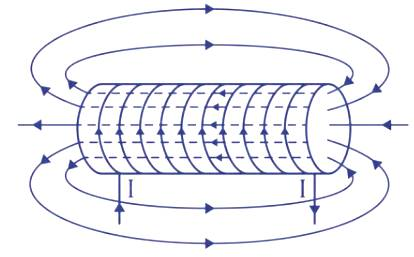
\includegraphics[scale=0.8]{../figs/VN11-PH-26-L-018-3-h91.jpg}
\end{center}
\subsection{Véctơ cảm ứng từ $\vec{B}$ do dòng điện chạy trong ống dây hình trụ}
Từ trường bên trong lòng ống dây mang dòng điện là từ trường đều. Vector cảm ứng từ tại một điểm trong lòng ống dây có đặc điểm: 
\begin{itemize}
	\item Điểm đặt: tại điểm đang xét.
	\item Phương: song song với trục của ống dây. 
	\item Chiều: xác định theo quy tắc nắm tay phải hoặc vào Nam ra Bắc.
	
	Nắm tay phải theo chiều dòng điện trong ống, khi đó ngón cái chỉ hướng của các đường cảm ứng từ nằm trong lòng ống dây.
	
	\item Độ lớn:  
	\begin{equation}
	B=4\pi\cdot 10^{-7}nI=4\pi\cdot 10^{-7}\dfrac{N}{l}I,
	\end{equation}
	trong đó,
	\begin{itemize}
		\item $N$ là số vòng dây.
		\item $I$ là cường độ của dòng điện, đơn vị ampère (A), 
		\item $l$ là là chiều dài ống dây, đơn vị mét (m),  
		\item $n$ là số vòng dây trên một mét chiều dài, có đơn vị là \SI{}{\per\meter}.
	\end{itemize}
	
\end{itemize}


\section{Bài tập}
\begin{dang}{Công thức cảm ứng từ $\vec{B}$ do dòng điện chạy trong ống dây hình trụ}
\end{dang}

\textbf{Phương pháp giải}

Áp dụng công thức $B=4\pi\cdot 10^{-7}nI=4\pi\cdot 10^{-7}\dfrac{N}{l}I$  , từ đó tìm được giá trị cảm ứng từ $B$, số vòng dây $N$ của ống dây, cường độ dòng điện $I$, $n$ số vòng dây trên một mét chiều dài, chiều dài $l$ của ống dây.

\luuy{Nếu các vòng dây quấn sát nhau thì số vòng trên một mét chiều dài ống dây $n=\dfrac{1}{d}$, trong đó, $d$ là đường kính của sợi dây.}




{\viduii{2}{	
Một dây dẫn đường kính tiết diện $d=\text{0,5}\ \text{mm}$ được phủ một lớp sơn cách điện mỏng và quấn thành một ống dây, các vòng dây quấn sát nhau. Cho dòng điện có cường độ $I=2\ \text{A}$ chạy qua ống dây. Xác định cảm ứng từ tại một điểm trên trục trong ống dây.
	\begin{mcq}(4)
		\item  $\text{2,5}\cdot 10^{-3}\ \text{T}$.
		\item  $\text{5}\cdot 10^{-3}\ \text{T}$.
		\item  $\text{7,5}\cdot 10^{-3}\ \text{T}$.
		\item  $\text{8,5}\cdot 10^{-3}\ \text{T}$.
	\end{mcq}
	}{
\begin{center}
		\textbf{Hướng dẫn giải:}
\end{center}
	
Do các vòng dây quấn sát nhau nên số vòng trên một mét chiều dài ống dây $n=\dfrac{1}{d}=2000\ \text{vòng/m}$.

Cảm ứng từ tại một điểm bên trong ống dây là $B=4\pi\cdot 10^{-7}nI=\text{5}\cdot 10^{-3}\ \text{T}$.
	
\textbf{	Đáp án: B.}
}}

{\viduii{2}{
	
Cho dòng điện cường độ $I=\text{0,15}\ \text{A}$ chạy qua các vòng dây của một ống dây thì cảm ứng từ bên trong ống dây là $\text{35}\cdot 10^{-5}\ \text{T}$. Ống dây dài 50 cm. Tính số vòng dây của ống dây.

	\begin{mcq}(4)
		\item $1858\ \text{vòng}$.
		\item $465\ \text{vòng}$.
		\item $1394\ \text{vòng}$.
		\item $929\ \text{vòng}$.
	\end{mcq}}
	{
\begin{center}
		\textbf{Hướng dẫn giải:}
\end{center}
	
	Cảm ứng từ bên trong ống dây là $B=4\pi\cdot 10^{-7}\dfrac{N}{l}I$.
	
	$\Rightarrow N=\dfrac{Bl}{4\pi\cdot 10^{-7}I}=929\ \text{vòng}$.
	
	Vậy số vòng dây của ống dây là $929\ \text{vòng}$.
	
\textbf{	Đáp án: D.}
	}
}

{\viduii{3}{	
Dùng một dây đồng có phủ một lớp sơn cách điện mỏng, quấn quanh một hình trụ dài $l=50\ \text{cm}$, có đường kính  $D=4\ \text{cm}$ để làm một ống dây. Sợi dây quấn ống dây có chiều dài $L=314\ \text{cm}$ và các vòng dây được quấn sát nhau. Hỏi nếu cho dòng điện cường độ $I=\text{0,4}\ \text{A}$ chạy qua ống dây, thì cảm ứng từ bên trong ống dây bằng bao nhiêu?
	\begin{mcq}(4)
		\item $\text{2,5}\cdot 10^{-5}\ \text{T}$.
		\item $\text{5}\cdot 10^{-5}\ \text{T}$.
		\item $\text{7,5}\cdot 10^{-5}\ \text{T}$.
		\item $\text{9,5}\cdot 10^{-5}\ \text{T}$.
	\end{mcq}}
	{
\begin{center}
		\textbf{Hướng dẫn giải:}
\end{center}
	
	Chu vi mỗi vòng dây là $\pi D$.
	
	Số vòng dây của ống dây: $N=\dfrac{L}{\pi D}$.
		
	Cảm ứng từ bên trong ống dây là $B=4\pi\cdot 10^{-7}\dfrac{N}{l}I=B=4\pi\cdot 10^{-7}\dfrac{L}{\pi Dl}I=\text{2,5}\cdot 10^{-5}\ \text{T}$.
		
\textbf{	Đáp án: A.}}
}




